\chapter{Score-Based Generative Modeling}
\label{chap:score_matching}

\section{The Geometry of Probability: Beyond the Partition Function}

The central ambition of generative modeling is to discover a mathematical representation of the underlying data distribution, $p_{\text{data}}(x)$, from which a given dataset $\mathcal{D} = \{x_1, \dots, x_N\}$ is assumed to be drawn independently and identically distributed. Historically, this endeavor has been dominated by the principle of maximum likelihood estimation (MLE). In the MLE paradigm, we posit a parameterized family of distributions $p_\theta(x)$ and seek the parameters $\theta$ that maximize the probability of the observed data.

However, the seemingly straightforward application of MLE is often frustrated by a fundamental architectural constraint. Many expressive families of probability distributions, particularly Energy-Based Models (EBMs), are defined up to an intractable normalization constant. An EBM defines the probability density as
\begin{equation}
    p_\theta(x) = \frac{e^{-E_\theta(x)}}{Z_\theta},
\end{equation}
where $E_\theta(x)$ is a parameterized scalar function referred to as the \textit{energy}, and $Z_\theta = \int e^{-E_\theta(x)} dx$ is the \textit{partition function}. The partition function ensures that the probability density integrates to one, a non-negotiable requirement of probability theory. Yet, computing $Z_\theta$ requires an integral over the entire high-dimensional data space $\mathcal{X}$, which is computationally prohibitive for spaces of even moderate dimensionality, such as images or text.

To bypass the partition function, we must shift our perspective from the absolute value of the probability density to its local geometry. Consider the spatial derivative of the log-probability density with respect to the data itself:
\begin{equation}
    \nabla_x \log p_\theta(x) = \nabla_x \left( -E_\theta(x) - \log Z_\theta \right) = -\nabla_x E_\theta(x).
\end{equation}
Because $Z_\theta$ is a constant with respect to $x$, its derivative vanishes. This vector field, $\nabla_x \log p(x)$, is known as the \textit{score function} (not to be confused with the Fisher score in statistics, which is the gradient with respect to the parameters $\theta$). 

The score function offers a profoundly different geometric interpretation of a probability distribution. While the density $p(x)$ assigns a scalar mass to every point in space, the score function assigns a vector pointing in the direction of the steepest ascent of the log-density. Intuitively, if one were placed at an arbitrary point in the data space, the score vector would indicate the direction to walk in order to reach more probable, "data-like" configurations. A generative model that accurately learns this vector field learns the fundamental structure of the data manifold. We can subsequently use this learned vector field to draw new samples by simulating a particle that stochastically follows the score vectors towards regions of high probability.

This approach, known as \textit{score-based generative modeling} or \textit{score matching}, liberates us from the tyranny of the partition function. We can train a neural network $s_\theta(x)$ to directly approximate the score function of the data distribution, $\nabla_x \log p_{\text{data}}(x)$, without ever explicitly modeling the density $p_\theta(x)$. However, a new challenge immediately arises: we do not have access to the true data score function $\nabla_x \log p_{\text{data}}(x)$. We only have empirical samples. The mathematical core of this chapter concerns how we can nonetheless train a network to match this unknown vector field.

\section{The Score Function and Fisher Divergence}

To formally learn the score function, we need an appropriate distance metric between our model's score $s_\theta(x)$ and the true data score $\nabla_x \log p_{\text{data}}(x)$. The natural choice is the expected squared Euclidean distance, a quantity deeply related to the Fisher divergence.

\begin{definition}[Fisher Divergence]
Let $P$ and $Q$ be two strictly positive, continuously differentiable probability distributions on $\mathbb{R}^d$. The Fisher divergence from $P$ to $Q$ is defined as
\begin{equation}
    D_F(P \parallel Q) = \mathbb{E}_{x \sim P} \left[ \left\| \nabla_x \log P(x) - \nabla_x \log Q(x) \right\|_2^2 \right].
\end{equation}
\end{definition}

In our context, we wish to minimize $J(\theta) = \frac{1}{2} D_F(p_{\text{data}} \parallel p_\theta)$, where we substitute a neural network $s_\theta(x)$ for $\nabla_x \log p_\theta(x)$. The explicit score matching objective is thus:
\begin{equation}
    J_{\text{ESM}}(\theta) = \frac{1}{2} \mathbb{E}_{x \sim p_{\text{data}}} \left[ \left\| s_\theta(x) - \nabla_x \log p_{\text{data}}(x) \right\|_2^2 \right].
\end{equation}
As noted, this objective is intractable because $\nabla_x \log p_{\text{data}}(x)$ is unknown. Remarkably, Aapo Hyvärinen demonstrated that this objective can be rewritten in a form that only depends on the data distribution via expectations over the samples, eliminating the need for the true score.

\begin{theorem}[Implicit Score Matching]
\label{thm:implicit_score_matching}
Assume that $p_{\text{data}}(x)$ is continuously differentiable and that $p_{\text{data}}(x) \|s_\theta(x)\|_2 \to 0$ as $\|x\|_2 \to \infty$. Then, minimizing $J_{\text{ESM}}(\theta)$ is equivalent to minimizing the implicit score matching objective $J_{\text{ISM}}(\theta)$, defined as:
\begin{equation}
    J_{\text{ISM}}(\theta) = \mathbb{E}_{x \sim p_{\text{data}}} \left[ \operatorname{tr}(\nabla_x s_\theta(x)) + \frac{1}{2} \|s_\theta(x)\|_2^2 \right],
\end{equation}
up to an additive constant that is independent of $\theta$. Here, $\nabla_x s_\theta(x)$ is the Jacobian matrix of the network, and $\operatorname{tr}$ denotes the trace operator.
\end{theorem}

\begin{proof}
We begin by expanding the squared Euclidean norm in the explicit score matching objective:
\begin{align*}
    J_{\text{ESM}}(\theta) &= \frac{1}{2} \int p_{\text{data}}(x) \left\| s_\theta(x) - \nabla_x \log p_{\text{data}}(x) \right\|_2^2 dx \\
    &= \int p_{\text{data}}(x) \left( \frac{1}{2}\|s_\theta(x)\|_2^2 - \langle s_\theta(x), \nabla_x \log p_{\text{data}}(x) \rangle + \frac{1}{2}\|\nabla_x \log p_{\text{data}}(x)\|_2^2 \right) dx.
\end{align*}
The third term $\frac{1}{2}\|\nabla_x \log p_{\text{data}}(x)\|_2^2$ is independent of $\theta$, so we can absorb it into a constant $C$. We now focus on the cross term:
\begin{align*}
    -\int p_{\text{data}}(x) \langle s_\theta(x), \nabla_x \log p_{\text{data}}(x) \rangle dx &= -\int p_{\text{data}}(x) \sum_{i=1}^d s_{\theta, i}(x) \frac{\partial}{\partial x_i} \log p_{\text{data}}(x) dx \\
    &= -\int \sum_{i=1}^d s_{\theta, i}(x) \frac{\partial}{\partial x_i} p_{\text{data}}(x) dx,
\end{align*}
where we utilized the identity $\nabla_x \log p(x) = \frac{\nabla_x p(x)}{p(x)}$.
We apply integration by parts to each dimension $i$:
\begin{equation}
    \int s_{\theta, i}(x) \frac{\partial}{\partial x_i} p_{\text{data}}(x) dx = \left[ s_{\theta, i}(x) p_{\text{data}}(x) \right]_{-\infty}^{\infty} - \int p_{\text{data}}(x) \frac{\partial}{\partial x_i} s_{\theta, i}(x) dx.
\end{equation}
By the assumption that $p_{\text{data}}(x) \|s_\theta(x)\|_2 \to 0$ as $x \to \pm\infty$, the boundary term evaluates to zero. Thus, the cross term simplifies to:
\begin{equation}
    \int \sum_{i=1}^d p_{\text{data}}(x) \frac{\partial}{\partial x_i} s_{\theta, i}(x) dx = \mathbb{E}_{x \sim p_{\text{data}}} \left[ \sum_{i=1}^d \frac{\partial s_{\theta, i}(x)}{\partial x_i} \right] = \mathbb{E}_{x \sim p_{\text{data}}} \left[ \operatorname{tr}(\nabla_x s_\theta(x)) \right].
\end{equation}
Substituting this back into the expanded objective yields $J_{\text{ISM}}(\theta) + C$, completing the proof.
\end{proof}

\begin{figure}[htbp]
\centering
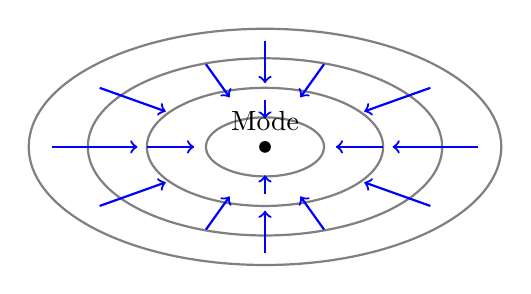
\begin{tikzpicture}[scale=1.5]
    % Draw some contours
    \draw[gray, thick] (0,0) ellipse (2 and 1);
    \draw[gray, thick] (0,0) ellipse (1.5 and 0.75);
    \draw[gray, thick] (0,0) ellipse (1 and 0.5);
    \draw[gray, thick] (0,0) ellipse (0.5 and 0.25);
    
    % Draw score vectors (gradient of log prob)
    \foreach \x/\y in {
        1.8/0, -1.8/0, 0/0.9, 0/-0.9,
        1.4/0.5, -1.4/-0.5, -1.4/0.5, 1.4/-0.5,
        1/0, -1/0, 0/0.4, 0/-0.4,
        0.5/0.7, -0.5/-0.7, 0.5/-0.7, -0.5/0.7
    } {
        \draw[->, blue, thick] (\x,\y) -- ({0.6*\x}, {0.6*\y});
    }
    
    \node[circle, fill=black, inner sep=1.5pt, label=above:Mode] at (0,0) {};
\end{tikzpicture}
\caption{The score function $\nabla_x \log p(x)$ forms a vector field that points toward the modes (regions of high density) of the probability distribution. The arrows are orthogonal to the level sets of the density.}
\label{fig:score_field}
\end{figure}

While Theorem \ref{thm:implicit_score_matching} provides a theoretically sound objective, it presents severe computational hurdles in the context of deep learning. The term $\operatorname{tr}(\nabla_x s_\theta(x))$ requires computing the trace of the Jacobian matrix of the network with respect to the inputs. For a $d$-dimensional input, this naïvely requires $d$ backward passes through the network. While Hutchinson's trace estimator can approximate this term, implicit score matching still struggles empirically, particularly because the objective provides poor learning signals in low-density regions where data samples are scarce.

\section{Denoising Score Matching}

To circumvent the computational cost of the Jacobian trace and provide a robust learning signal everywhere, Vincent (2011) introduced Denoising Score Matching (DSM). The core insight is that adding a small amount of noise to the data smooths out the distribution, filling in low-density regions, and profoundly simplifying the score matching objective.

Let us define a predefined noise distribution $q_\sigma(\tilde{x}|x) = \mathcal{N}(\tilde{x}; x, \sigma^2 I)$. The perturbed data distribution is the marginal:
\begin{equation}
    q_\sigma(\tilde{x}) = \int q_\sigma(\tilde{x}|x) p_{\text{data}}(x) dx.
\end{equation}
Instead of matching the score of the original data, we aim to match the score of this perturbed distribution, $\nabla_{\tilde{x}} \log q_\sigma(\tilde{x})$.

\begin{theorem}[Denoising Score Matching]
\label{thm:denoising_score_matching}
Minimizing the explicit score matching objective for the perturbed distribution $q_\sigma(\tilde{x})$:
\begin{equation}
    J_{\text{SM}}(\theta; \sigma) = \frac{1}{2} \mathbb{E}_{\tilde{x} \sim q_\sigma(\tilde{x})} \left[ \left\| s_\theta(\tilde{x}) - \nabla_{\tilde{x}} \log q_\sigma(\tilde{x}) \right\|_2^2 \right],
\end{equation}
is equivalent to minimizing the denoising score matching objective:
\begin{equation}
    J_{\text{DSM}}(\theta; \sigma) = \frac{1}{2} \mathbb{E}_{x \sim p_{\text{data}}} \mathbb{E}_{\tilde{x} \sim q_\sigma(\tilde{x}|x)} \left[ \left\| s_\theta(\tilde{x}) - \nabla_{\tilde{x}} \log q_\sigma(\tilde{x}|x) \right\|_2^2 \right],
\end{equation}
up to an additive constant independent of $\theta$.
\end{theorem}

\begin{proof}
We expand $J_{\text{SM}}(\theta; \sigma)$:
\begin{equation}
    J_{\text{SM}}(\theta; \sigma) = \frac{1}{2} \mathbb{E}_{q_\sigma(\tilde{x})} [\|s_\theta(\tilde{x})\|_2^2] - \mathbb{E}_{q_\sigma(\tilde{x})} [\langle s_\theta(\tilde{x}), \nabla_{\tilde{x}} \log q_\sigma(\tilde{x}) \rangle] + C_1.
\end{equation}
Let us focus on the cross term. Using the identity $q_\sigma(\tilde{x}) \nabla_{\tilde{x}} \log q_\sigma(\tilde{x}) = \nabla_{\tilde{x}} q_\sigma(\tilde{x})$, we have:
\begin{align*}
    \mathbb{E}_{q_\sigma(\tilde{x})} [\langle s_\theta(\tilde{x}), \nabla_{\tilde{x}} \log q_\sigma(\tilde{x}) \rangle] &= \int \langle s_\theta(\tilde{x}), \nabla_{\tilde{x}} q_\sigma(\tilde{x}) \rangle d\tilde{x} \\
    &= \int \left\langle s_\theta(\tilde{x}), \nabla_{\tilde{x}} \int p_{\text{data}}(x) q_\sigma(\tilde{x}|x) dx \right\rangle d\tilde{x} \\
    &= \iint p_{\text{data}}(x) \langle s_\theta(\tilde{x}), \nabla_{\tilde{x}} q_\sigma(\tilde{x}|x) \rangle dx d\tilde{x} \\
    &= \iint p_{\text{data}}(x) q_\sigma(\tilde{x}|x) \langle s_\theta(\tilde{x}), \nabla_{\tilde{x}} \log q_\sigma(\tilde{x}|x) \rangle dx d\tilde{x} \\
    &= \mathbb{E}_{x \sim p_{\text{data}}} \mathbb{E}_{\tilde{x} \sim q_\sigma(\tilde{x}|x)} [\langle s_\theta(\tilde{x}), \nabla_{\tilde{x}} \log q_\sigma(\tilde{x}|x) \rangle].
\end{align*}
Now, consider the expansion of $J_{\text{DSM}}(\theta; \sigma)$:
\begin{equation}
    J_{\text{DSM}}(\theta; \sigma) = \frac{1}{2} \mathbb{E}_{x, \tilde{x}} [\|s_\theta(\tilde{x})\|_2^2] - \mathbb{E}_{x, \tilde{x}} [\langle s_\theta(\tilde{x}), \nabla_{\tilde{x}} \log q_\sigma(\tilde{x}|x) \rangle] + C_2.
\end{equation}
Because the marginal of $\tilde{x}$ over the joint distribution is $q_\sigma(\tilde{x})$, the first term $\mathbb{E}_{x, \tilde{x}} [\|s_\theta(\tilde{x})\|_2^2]$ is identical to $\mathbb{E}_{q_\sigma(\tilde{x})} [\|s_\theta(\tilde{x})\|_2^2]$. Since we have shown the cross terms are also equivalent, the two objectives differ only by a constant $(C_1 - C_2)$ that does not depend on $\theta$.
\end{proof}

\begin{figure}[htbp]
\centering
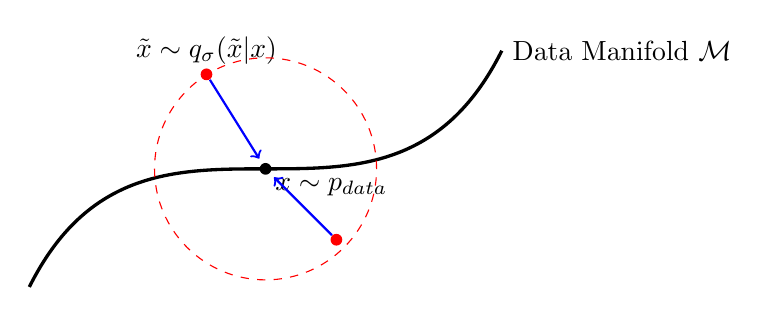
\begin{tikzpicture}[scale=1.5]
    % Data manifold (a curve)
    \draw[very thick, black] (-2, -1) .. controls (-1, 1) and (1, -1) .. (2, 1) node[right] {Data Manifold $\mathcal{M}$};
    
    % Points on manifold
    \node[circle, fill=black, inner sep=1.5pt] (x) at (0, 0) {};
    \node[below right] at (x) {$x \sim p_{\text{data}}$};
    
    % Corrupted points
    \node[circle, fill=red, inner sep=1.5pt] (xtilde1) at (-0.5, 0.8) {};
    \node[above] at (xtilde1) {$\tilde{x} \sim q_\sigma(\tilde{x}|x)$};
    
    \node[circle, fill=red, inner sep=1.5pt] (xtilde2) at (0.6, -0.6) {};
    
    % Arrows from corrupted points back to manifold (score)
    \draw[->, blue, thick, shorten >= 2pt] (xtilde1) -- (x);
    \draw[->, blue, thick, shorten >= 2pt] (xtilde2) -- (x);
    
    % Noise distribution circle
    \draw[dashed, red] (x) circle (0.94); % 0.94 is roughly distance to xtilde1
\end{tikzpicture}
\caption{Denoising Score Matching. Clean data points $x$ on a low-dimensional manifold are perturbed to $\tilde{x}$. Because the noise distribution $q_\sigma(\tilde{x}|x)$ is Gaussian, its score $\nabla_{\tilde{x}} \log q_\sigma(\tilde{x}|x) = (x - \tilde{x}) / \sigma^2$ is a vector pointing exactly from the noisy point back to the clean point. The network learns to act as a denoiser.}
\label{fig:denoising}
\end{figure}

The brilliance of DSM lies in the analytical tractability of the conditional score. For Gaussian noise $q_\sigma(\tilde{x}|x) \propto \exp(-\frac{\|\tilde{x} - x\|_2^2}{2\sigma^2})$, the conditional score is simply:
\begin{equation}
    \nabla_{\tilde{x}} \log q_\sigma(\tilde{x}|x) = -\frac{\tilde{x} - x}{\sigma^2}.
\end{equation}
Substituting this into $J_{\text{DSM}}$, the objective becomes a simple mean squared error between the network's output and the noise vectors. The network acts as a vector field pointing from perturbed points back towards their clean origins on the data manifold, effectively functioning as a denoiser.

\section{Numerical Example: Isotropic Gaussian}

To build intuition, let us derive the true score for a simple case and observe what the network must learn. Consider a target distribution that is an isotropic Gaussian, $p_{\text{data}}(x) = \mathcal{N}(x; \mu, \sigma_d^2 I)$. 

The density is:
\begin{equation}
    p_{\text{data}}(x) = \frac{1}{(2\pi \sigma_d^2)^{d/2}} \exp\left( -\frac{\|x - \mu\|_2^2}{2\sigma_d^2} \right).
\end{equation}
Taking the logarithm:
\begin{equation}
    \log p_{\text{data}}(x) = -\frac{\|x - \mu\|_2^2}{2\sigma_d^2} - \frac{d}{2} \log(2\pi \sigma_d^2).
\end{equation}
The true score function is the gradient:
\begin{equation}
    \nabla_x \log p_{\text{data}}(x) = -\frac{x - \mu}{\sigma_d^2}.
\end{equation}
This is a linear vector field pointing precisely towards the mean $\mu$, with a magnitude proportional to the distance from the mean, scaled inversely by the variance. If we parameterize a neural network $s_\theta(x) = W x + b$, implicit score matching would recover $W = -\frac{1}{\sigma_d^2}I$ and $b = \frac{\mu}{\sigma_d^2}$. 

\begin{horizon}
The mathematical equivalence of Denoising Score Matching implies a profound connection between score functions and information theory, crystallized in the celebrated de Bruijn identity. The identity states that the derivative of the Shannon differential entropy of a random variable undergoing Gaussian diffusion is precisely proportional to its Fisher information: $\frac{d}{d\sigma^2} h(X + \mathcal{N}(0, \sigma^2 I)) = \frac{1}{2} J(X + \mathcal{N}(0, \sigma^2 I))$. 

It is conjectured that the empirical success of multi-scale score matching (using an annealed noise schedule $\sigma_1 > \sigma_2 > \dots > \sigma_L$) is not merely a numerical trick, but fundamentally tied to the optimal transport of information. Future work might show that the optimal noise schedule for training diffusion models rigorously minimizes the rate of information loss per step, mapping exactly onto bounds derived in non-equilibrium thermodynamics for the minimal dissipation of work. An open question is whether the Information Bottleneck principle can be explicitly embedded into the score matching objective to bound the generalization error of generative sampling.
\end{horizon}

\section{Summary}
In this chapter, we explored the paradigm of score-based generative modeling, which shifts the focus from estimating normalized probability densities to estimating the score function—the gradient of the log-density. This sidesteps the intractable partition function. We proved that while direct score matching requires computationally expensive trace operations (Implicit Score Matching), the objective can be elegantly reformulated into Denoising Score Matching. By adding Gaussian noise, the network learns to denoise, which corresponds exactly to estimating the score of the smoothed data distribution. This mathematical framework provides the critical foundation for the continuous-time diffusion models explored in subsequent chapters.

\section*{Exercises}
\begin{enumerate}
    \item \textbf{Jacobian Trace for Multilayer Perceptrons.} Consider a 2-layer MLP $s_\theta(x) = W_2 \phi(W_1 x + b_1) + b_2$ where $\phi$ is an element-wise activation function. Derive the analytical expression for the trace term $\operatorname{tr}(\nabla_x s_\theta(x))$ required in Implicit Score Matching. What is the computational complexity compared to evaluating $s_\theta(x)$?
    \item \textbf{Score of a Gaussian Mixture.} Let $p(x) = \frac{1}{2}\mathcal{N}(x; \mu_1, \Sigma_1) + \frac{1}{2}\mathcal{N}(x; \mu_2, \Sigma_2)$. Compute the exact score function $\nabla_x \log p(x)$. Show analytically that the score function evaluates to a non-linear combination of the individual cluster scores, heavily weighted towards the nearest cluster mode.
    \item \textbf{Variance of the DSM Estimator.} While Denoising Score Matching is unbiased with respect to the explicit score matching gradient, its empirical variance can be high for small $\sigma$. Prove that as $\sigma \to 0$, the variance of the stochastic gradient of $J_{\text{DSM}}$ approaches infinity, explaining the necessity of perturbing the data significantly during training.
\end{enumerate}

% TODO-CITE: Ensure all named results are cited.
